\documentclass[11pt]{article}

% ACL style: needs acl.sty from the official ACL template; the bibliography is inside this file
% (https://github.com/acl-org/acl-style-files). "final" shows the authors;
% "review" anonymises the paper and adds line numbers.
% Numbered citations [1], [2-4]: load natbib in numeric mode before acl.sty,
% and keep natbib's numbered reference list (acl.sty would otherwise print it without numbers).
\usepackage[numbers,square,sort&compress]{natbib}
\makeatletter
\let\numthebibliography\thebibliography
\let\endnumthebibliography\endthebibliography
\makeatother
\usepackage[final]{acl}
\makeatletter
\let\thebibliography\numthebibliography
\let\endthebibliography\endnumthebibliography
\makeatother
\usepackage{times}
\usepackage{latexsym}
\usepackage[T1]{fontenc}
\usepackage[utf8]{inputenc}
\usepackage{microtype}
\usepackage{inconsolata}
\usepackage{booktabs}
\usepackage{tabularx}
\usepackage{amsmath}
\usepackage{amssymb}
\usepackage{graphicx}

% ============================================================
% TITLE AND AUTHORS
% ============================================================

\title{EcoExplain-VLM: A Benchmark for Classifying and
Explaining Forest Vegetation Change with Vision-Language Models}

\author{
  Rama Chandra Prasad Pillutla \and Chinta Phani Rama Vaibhav \and Shaik Afzal Basha \\
  {\normalsize\mdseries Lab for Spatial Informatics} \\
  {\normalsize\mdseries International Institute of Information Technology Hyderabad, India} \\
  {\normalsize\mdseries\texttt{rcprasad@iiit.ac.in}, \texttt{chinta.vaibhav@students.iiit.ac.in},} \\
  {\normalsize\mdseries\texttt{afzalbasha.shaik@students.iiit.ac.in}}
}

\begin{document}

\maketitle

% ============================================================
% ABSTRACT
% ============================================================

\begin{abstract}
Vision-language models (VLMs) promise to turn multi-sensor satellite
evidence into decisions that people can read and check. We introduce
EcoExplain-VLM, a benchmark of 366 forest patches in Kanha Tiger
Reserve, India, that pairs matched dry-season Sentinel-2 images
(January-February 2022 and 2023) with an evidence card summarising
Sentinel-2 indices, Sentinel-1 backscatter, CHIRPS rainfall, ERA5-Land
anomalies and NASADEM terrain. Each patch carries a three-class
vegetation-change label (decline, stable, increase) derived from NDVI
change, and every model is tested on the same 55 held-out patches. A
central contribution is a leakage-controlled protocol. With the original
card, whose final summary line restates the label, Qwen2-VL-2B reaches
56.4\% zero-shot; when that line is removed and all models receive the
same numeric table, Qwen2-VL-2B scores 32.7\% and the best model,
LLaVA-Interleave-0.5B, 43.6\%, close to the 34.5\% majority baseline. A
balanced, label-free LoRA on 16 patches gives 36.4\%, whereas a
one-number NDVI threshold reaches 94.5\%, showing that the evidence is
sufficient and that small VLMs do not yet exploit it. For explanations,
a structured cite-only prompt makes 75.8\% (Qwen2-VL-2B) and 71.1\%
(LLaVA) of checkable claims agree with the measured changes, and an
explanation-tuned Qwen2-VL-2B separates decline from increase (61.8\%,
significantly above the majority baseline). The benchmark, protocol and
code provide a reproducible basis for developing evidence-grounded VLMs
for forest monitoring.
\end{abstract}

\noindent\textbf{Keywords:} vision-language models; forest vegetation
change; multi-source remote sensing; Sentinel-2; Sentinel-1 SAR;
evaluation leakage; LoRA; evidence-grounded explanation; Kanha Tiger
Reserve

% ============================================================
% 1. INTRODUCTION
% ============================================================

\section{Introduction}

India's protected forests are tracked using various satellite products and evaluation methods. 
Global forest-change maps \citep{hansen2013}, time-series analysis and radar-based disturbance alerts now effectively detect vegetation changes. 
These solutions sometimes lack a concise and verifiable explanation of the change, which is important for forest managers and policymakers.For small variations in vegetation, such as those caused by drought or grazing, the evidence is often subtle and distributed across multiple sources.

Vision-language models offer a natural way to provide them. They read
images and text together and answer in free language \citep{wang2024qwen2vl,li2024interleave}, and remote-sensing variants already
answer questions about overhead imagery, caption
changes between image pairs and ground their
answers spatially \citep{kuckreja2024}. A VLM can potentially classify forest changes and explain its predictions using before-and-after images and summarized optical, radar, climate, and terrain data.


Four characteristics of existing models necessitate thorough assessment. 
Firstly, VLMs have the capability to articulate information that isn’t included in the input. 
Secondly, a coherent explanation doesn’t always equate to an accurate one: the reasons provided may not represent how the model derived its conclusion \citep{jacovi2020}.
Thirdly, smaller models are highly influenced by the phrasing of prompts and have consistent response tendencies. 
 A further concern relates to the benchmark itself: if any component of the input discloses the answer, measuring accuracy assesses the ability to retrieve that information rather than the actual intended skill \citep{kaufman2012}.
Consequently, a valuable benchmark for evidence-based VLMs must manage what the model perceives and evaluate its outputs.

This paper presents EcoExplain-VLM, a benchmark and evaluation protocol
built for that purpose in Kanha Tiger Reserve, central India. We ask
three questions:
\begin{enumerate}
\item Can open VLMs with 0.5-3 billion parameters classify relative
vegetation change from before/after images and multi-sensor evidence
without task-specific training, and how does the answer depend on what
the evidence card contains?
\item Does a small, class-balanced LoRA fine-tune \citep{hu2022lora}
change that ability when the label cannot be read from the input?
\item When prompted to explain their responses, do the models provide justifications that align with the observed changes, and what impact do the arrangement of prompts and fine-tuning on justifications have on that alignment?
\end{enumerate}

Our contributions are fourfold:

1. A reproducible benchmark comprising 366 patches from five data sources, with matched dry-season windows, fixed data splits, and an additional spatial block split.

2. A leakage-controlled evaluation protocol that reruns key experiments without the card’s summary line and uses identical inputs across models to quantify its influence on apparent zero-shot performance.

3. An automated claim-verification method that evaluates directional statements in explanations against measured changes, combined with a structured cite-only prompt that achieves 71--76\% claim correctness

4. Fine-tuning experiments that establish baselines for future research, including an explanation-tuned model capable of distinguishing forest decline from increase without access to the label.

% ============================================================
% 2. DATA AND METHODS
% ============================================================

\section{Data and Methods}
\label{sec:methods}

\subsection{Study Area}

Kanha Tiger Reserve lies in the Maikal hills of central India, in the
Mandla and Balaghat districts of Madhya Pradesh. Its core zone covers
917.44\,km$^2$ and its buffer zone 1,134.36\,km$^2$, 2,051.79\,km$^2$ in
total. The forests are dominated by sal
(\emph{Shorea robusta}) with moist and dry mixed deciduous forest and
grassland meadows. Most rain falls in the
June-September monsoon, and January-February is cool, dry and largely
cloud-free, which makes it well suited to optical comparison between
years.

All processing used a rectangle enclosing the reserve,
80.433\textdegree-81.050\textdegree\,E and
22.117\textdegree-22.450\textdegree\,N (2,350.7\,km$^2$). Because the
rectangle is larger than the gazetted reserve, some patches lie in the
buffer zone or just outside the boundary. The 1,200 candidate patch
centres from which the dataset was drawn all fall inside the rectangle;
the pool contains an empty strip near 80.75-80.85\textdegree\,E whose
origin was not recorded.

% Add the study-area map here: India (official boundary, untrimmed),
% Madhya Pradesh, the reserve and the rectangle with patch points.
% \begin{figure*}[t]
%   \centering
%   \includegraphics[width=\textwidth]{figures/fig_study_area.png}
%   \caption{Study area. (a) India; (b) Madhya Pradesh and Kanha Tiger
%   Reserve; (c) the 366 patches by class.}
%   \label{fig:studyarea}
% \end{figure*}

\subsection{Data Sources}

\subsubsection{Optical and Synthetic Aperture Radar Data}

Sentinel-2 Level-2A surface reflectance \citep{drusch2012} was taken
from the harmonized Earth Engine collection, which removes the offset
introduced by the processing-baseline change of 25 January 2022. Scenes
with more than 20\% cloud were discarded, clouds, cirrus and shadows were
masked with the Scene Classification Layer, and per-pixel median
composites were formed for T0 (1 January-28 February 2022; 20 scenes)
and T1 (the same window in 2023; 23 scenes). From each composite we
computed four indices, NDVI \citep{tucker1979}, EVI, NDMI and NBR:
\begin{align}
\mathrm{NDVI} &= \frac{\rho_{\mathrm{NIR}}-\rho_{\mathrm{Red}}}{\rho_{\mathrm{NIR}}+\rho_{\mathrm{Red}}}, \label{eq:ndvi}\\
\mathrm{EVI} &= 2.5\,\frac{\rho_{\mathrm{NIR}}-\rho_{\mathrm{Red}}}{\rho_{\mathrm{NIR}}+6\rho_{\mathrm{Red}}-7.5\rho_{\mathrm{Blue}}+1}, \label{eq:evi}\\
\mathrm{NDMI} &= \frac{\rho_{\mathrm{NIR}}-\rho_{\mathrm{SWIR1}}}{\rho_{\mathrm{NIR}}+\rho_{\mathrm{SWIR1}}}, \label{eq:ndmi}\\
\mathrm{NBR} &= \frac{\rho_{\mathrm{NIR}}-\rho_{\mathrm{SWIR2}}}{\rho_{\mathrm{NIR}}+\rho_{\mathrm{SWIR2}}}, \label{eq:nbr}
\end{align}
Change is defined as
\begin{equation}
\Delta I = I_{T1}-I_{T0},
\label{eq:delta}
\end{equation}
so a negative $\Delta\mathrm{NDVI}$ means less greenness in 2023. A
true-colour RGB chip was rendered for each window as the visual input to
the VLMs.

Sentinel-1 GRD C-band backscatter was composited for
the same windows from the dominant (descending) orbit direction (15
scenes at T0, 20 at T1; only Sentinel-1A was operating in both windows).
The VV and VH channels respond to canopy structure and moisture and are
unaffected by cloud. All compositing and export ran in Google Earth
Engine \citep{gorelick2017}.

\subsubsection{Ancillary Environmental Data}

Daily rainfall data from CHIRPS was aggregated over each 58-day period. Monthly 2\,m air temperature and top-layer soil moisture data were obtained from ERA5-Land, which we then transformed into month-matched anomalies based on a 2015-2021 climatology:  
\begin{equation}  
A=\tfrac{1}{2}\sum_{m\in\{\mathrm{Jan},\mathrm{Feb}\}}\left(\overline{X}_{m,\mathrm{window}}-\overline{X}_{m,2015\text{-}2021}\right).  
\label{eq:anomaly}  
\end{equation}  
Elevation, slope, and aspect at a 30\,m resolution were provided by NASADEM. While these layers are not included in the label, they are referenced in explanations concerning drought or terrain when appropriate evidence is available. Table~\ref{tab:sources} provides a summary of the five data sources.

\begin{table}[t]
\centering
\small
\begin{tabularx}{\columnwidth}{lXl}
\toprule
Source & Variables & Resolution \\
\midrule
Sentinel-2 L2A & 10 bands; NDVI, EVI, NDMI, NBR & 10-20\,m \\
Sentinel-1 GRD & VV, VH (dB), descending & 10\,m \\
CHIRPS & window rainfall total & $\approx$5.5\,km \\
ERA5-Land & temperature, soil-moisture anomalies & $\approx$9\,km \\
NASADEM & elevation, slope, aspect & 30\,m \\
\bottomrule
\end{tabularx}
\caption{The five data sources, all accessed through Google Earth Engine.}
\label{tab:sources}
\end{table}

\subsection{Preprocessing and Patch Generation}
Each patch is the bounding square of a 320 m circle around a candidate center (64 pixels of 10 m), trimmed to the study rectangle. The export uses geographic coordinates (EPSG:4326), with typical patches measuring approximately 70\,$\times$\,65 pixels. Each patch exported 15 rasters, totaling 5,490 files. Candidates with masked fractions above 0.15 in either year were removed, whereas selected patches had masked fractions ranging from 0.8\% to 2.3\%.


To create VLMs, each RGB chip was padded to a square and extended to a 512\,$\times$\,512 canvas. Physical layers were stored as arrays on the same canvas. Otsu thresholding of $\Delta$NDVI and $\Delta$NBR identified potential disturbance boxes, which were only preserved for three patches due to a quality policy. Selected patch centers are at least 639 m apart (median nearest-neighbor distance: 1,430 m).

\subsection{Change Evidence and Labelling}

Let $\Delta$ denote the patch-mean NDVI change and $q_{15}=-0.0377$,
$q_{85}=+0.0031$ its 15th and 85th percentiles over the 1,200-patch pool.
Following the roadmap's recommendation to use region-specific quantiles,
the automatic label is
\begin{equation}
\mathrm{class}=
\begin{cases}
\text{uncertain} & \text{masked}>0.15,\\
\text{decline} & \Delta\le q_{15},\\
\text{increase} & \Delta\ge q_{85},\\
\text{stable} & \text{otherwise.}
\end{cases}
\label{eq:label}
\end{equation}
Uncertain patches were not sampled. The final dataset holds 366 patches:
120 decline, 124 stable and 122 increase. The region as a whole lost a
little greenness between the two years (mean $\Delta=-0.016$, s.d.\
0.027), so the classes are relative ranks for this reserve and pair of
years: ``decline'' marks the 15\% of patches that lost most greenness
and ``increase'' the 15\% that fared best. Only 34 patches changed NDVI
by 0.05 or more. One annotator assigned a reference class to 19 patches,
agreeing with the automatic label on 8 (42\%; Wilson 95\% interval
23-64\%).

Each patch also has a structured evidence card, generated from its
rasters, that lists index values and changes, radar means, rainfall,
climate anomalies and terrain. In the original pipeline the card ends
with a one-line summary, ``Inference for \ldots: vegetation\_trend=\ldots,
candidate\_class=\ldots'', which restates the card's trend word and the
label. Section~\ref{sec:protocol} describes how the evaluation controls
for this line.

\subsection{Dataset Construction and Data Splits}

Records are stored as JSON Lines without coordinates. The patches were
split by class-stratified random sampling (seed 42) into 256 training,
55 development and 55 test patches; the test set holds 18 decline, 18
stable and 19 increase patches, so always predicting ``increase'' gives
a majority baseline of 34.5\%. All results below use this test set. Because
random splits of spatial data can overstate accuracy, we also provide a spatial block split in
which whole blocks of a 5\,$\times$\,4 grid are held out (266/46/54
patches).

\subsection{Vision-Language Model Evaluation}

\subsubsection{Models}

We compare four instruction-tuned open checkpoints (Table~\ref{tab:models}):
Qwen2-VL-2B-Instruct \citep{wang2024qwen2vl}, LLaVA-NeXT-Interleave
0.5B \citep{li2024interleave}, PaliGemma-3B-mix-224
and BLIP-2 OPT-2.7B. Decoding is greedy,
and a deterministic parser maps each answer to a class, ignoring text
that merely repeats the instruction.

\begin{table}[t]
\centering
\small
\begin{tabularx}{\columnwidth}{lXr}
\toprule
Model & Image encoder / language model & Size \\
\midrule
Qwen2-VL-2B & dynamic-resolution ViT / Qwen2 & 2B \\
LLaVA-Interleave & SigLIP / Qwen1.5-0.5B & 0.5B \\
PaliGemma & SigLIP / Gemma & 3B \\
BLIP-2 OPT & ViT + Q-Former / OPT-2.7B & 3.8B \\
\bottomrule
\end{tabularx}
\caption{The four models (Hugging Face checkpoints).}
\label{tab:models}
\end{table}

\subsubsection{Input Protocols}
\label{sec:protocol}

Every model receives the T0 and T1 chips and is asked for one word:
\texttt{decline}, \texttt{increase} or \texttt{stable}. Three text inputs
were used:
\begin{itemize}
\item \textbf{Full card} (``Condition~C''): the complete evidence card,
including the summary line. Qwen2-VL-2B and LLaVA received the full
card; PaliGemma, which declines long prompts, received its NDVI line;
BLIP-2, which accepts a single image, received the two chips side by
side with a short prompt.
\item \textbf{Evidence-only}: the full card with the summary line and
all label words removed.
\item \textbf{Compact}: a label-free numeric table of the measured
changes, identical for every model.
\end{itemize}
The evidence-only and compact protocols are leak-free \citep{kaufman2012}, and the compact
protocol is also input-equal across models. A script verifies that no
leak-free prompt contains the label. As reference points we report the
majority baseline and a threshold rule on the card's $\Delta$NDVI value,
with cut-offs either fixed at $\pm0.02$ or fitted on the training split.

\subsubsection{Parameter-Efficient Fine-Tuning}

We fine-tune Qwen2-VL-2B with LoRA \citep{hu2022lora}, which adds a
trainable low-rank update to frozen weights,
\begin{equation}
W = W_0 + \frac{\alpha}{r}BA,
\label{eq:lora}
\end{equation}
with rank $r=8$, $\alpha=16$ and dropout 0.1 on all attention and MLP
projections. The base model is stored in 4 bits
and trained with AdamW (learning rate
$5\times10^{-5}$, weight decay 0.05, gradient accumulation over four
steps) on an NVIDIA GTX 1080 Ti. Two adapters are reported.

The \textbf{class LoRA} is trained for one epoch on 16 training patches
drawn evenly across classes (6 decline, 5 stable, 5 increase) with the
evidence-only card at training and test time. The \textbf{explanation
LoRA} follows a teacher-student design: Qwen2-VL-2B wrote a JSON
justification for each training patch from the compact table, and a
justification was kept only if its class was correct, it contained at
least two checkable claims and all of them agreed with the measured
changes. Of 256 justifications, 28 passed; the 16 that fell within the
first 128 training patches were used for one epoch.

\subsubsection{Evaluation Metrics}

Classification is scored by accuracy and macro-F1,
\begin{equation}
\mathrm{Acc}=\frac{\#\text{correct}}{N},\qquad
\text{macro-F1}=\frac{1}{3}\sum_{c}F1_c,
\label{eq:metrics}
\end{equation}
with Wilson 95\% intervals,
\begin{equation}
\frac{\hat p+\frac{z^2}{2n}}{1+\frac{z^2}{n}}\pm\frac{z}{1+\frac{z^2}{n}}\sqrt{\frac{\hat p(1-\hat p)}{n}+\frac{z^2}{4n^2}},
\label{eq:wilson}
\end{equation}
and paired comparisons by McNemar's exact test.

Explanations are scored automatically. The scorer finds each indicator
(NDVI, EVI, NDMI, NBR, green cover, VV, VH, rainfall, soil moisture,
temperature) and its nearest direction word, converts the measured change
into a direction with an indicator-specific dead-band $\tau$ (0.02 for
the indices),
\begin{equation}
\mathrm{dir}(\Delta)=
\begin{cases}
\text{stable} & |\Delta|<\tau,\\
\text{increase} & \Delta\ge\tau,\\
\text{decrease} & \Delta\le-\tau,
\end{cases}
\label{eq:deadband}
\end{equation}
and counts a claim as correct when the two directions match. We report
the share of correct claims, the share of explanations with at least one
incorrect claim, and self-consistency (whether the dominant claimed
direction agrees with the model's own class). This measures consistency
with the evidence rather than faithfulness to the model's internal
reasoning \citep{jacovi2020}; ROUGE-L is reported
only as a measure of copying.

\subsection{Experimental Workflow}

Figure~\ref{fig:workflow} summarises the workflow in six steps: (1)
study design with matched windows; (2) collection of the five sources;
(3) compositing and export in Earth Engine; (4) image processing,
labelling and evidence cards; (5) freezing of the dataset and splits; and
(6) three evaluation tracks on the same 55 test patches: zero-shot
classification (Track~A), class LoRA (Track~B) and explanations
(Track~C). The development set was used only for prompt wording, the
closed-set probe's bias and checkpoint selection.

\begin{figure*}[t]
\centering
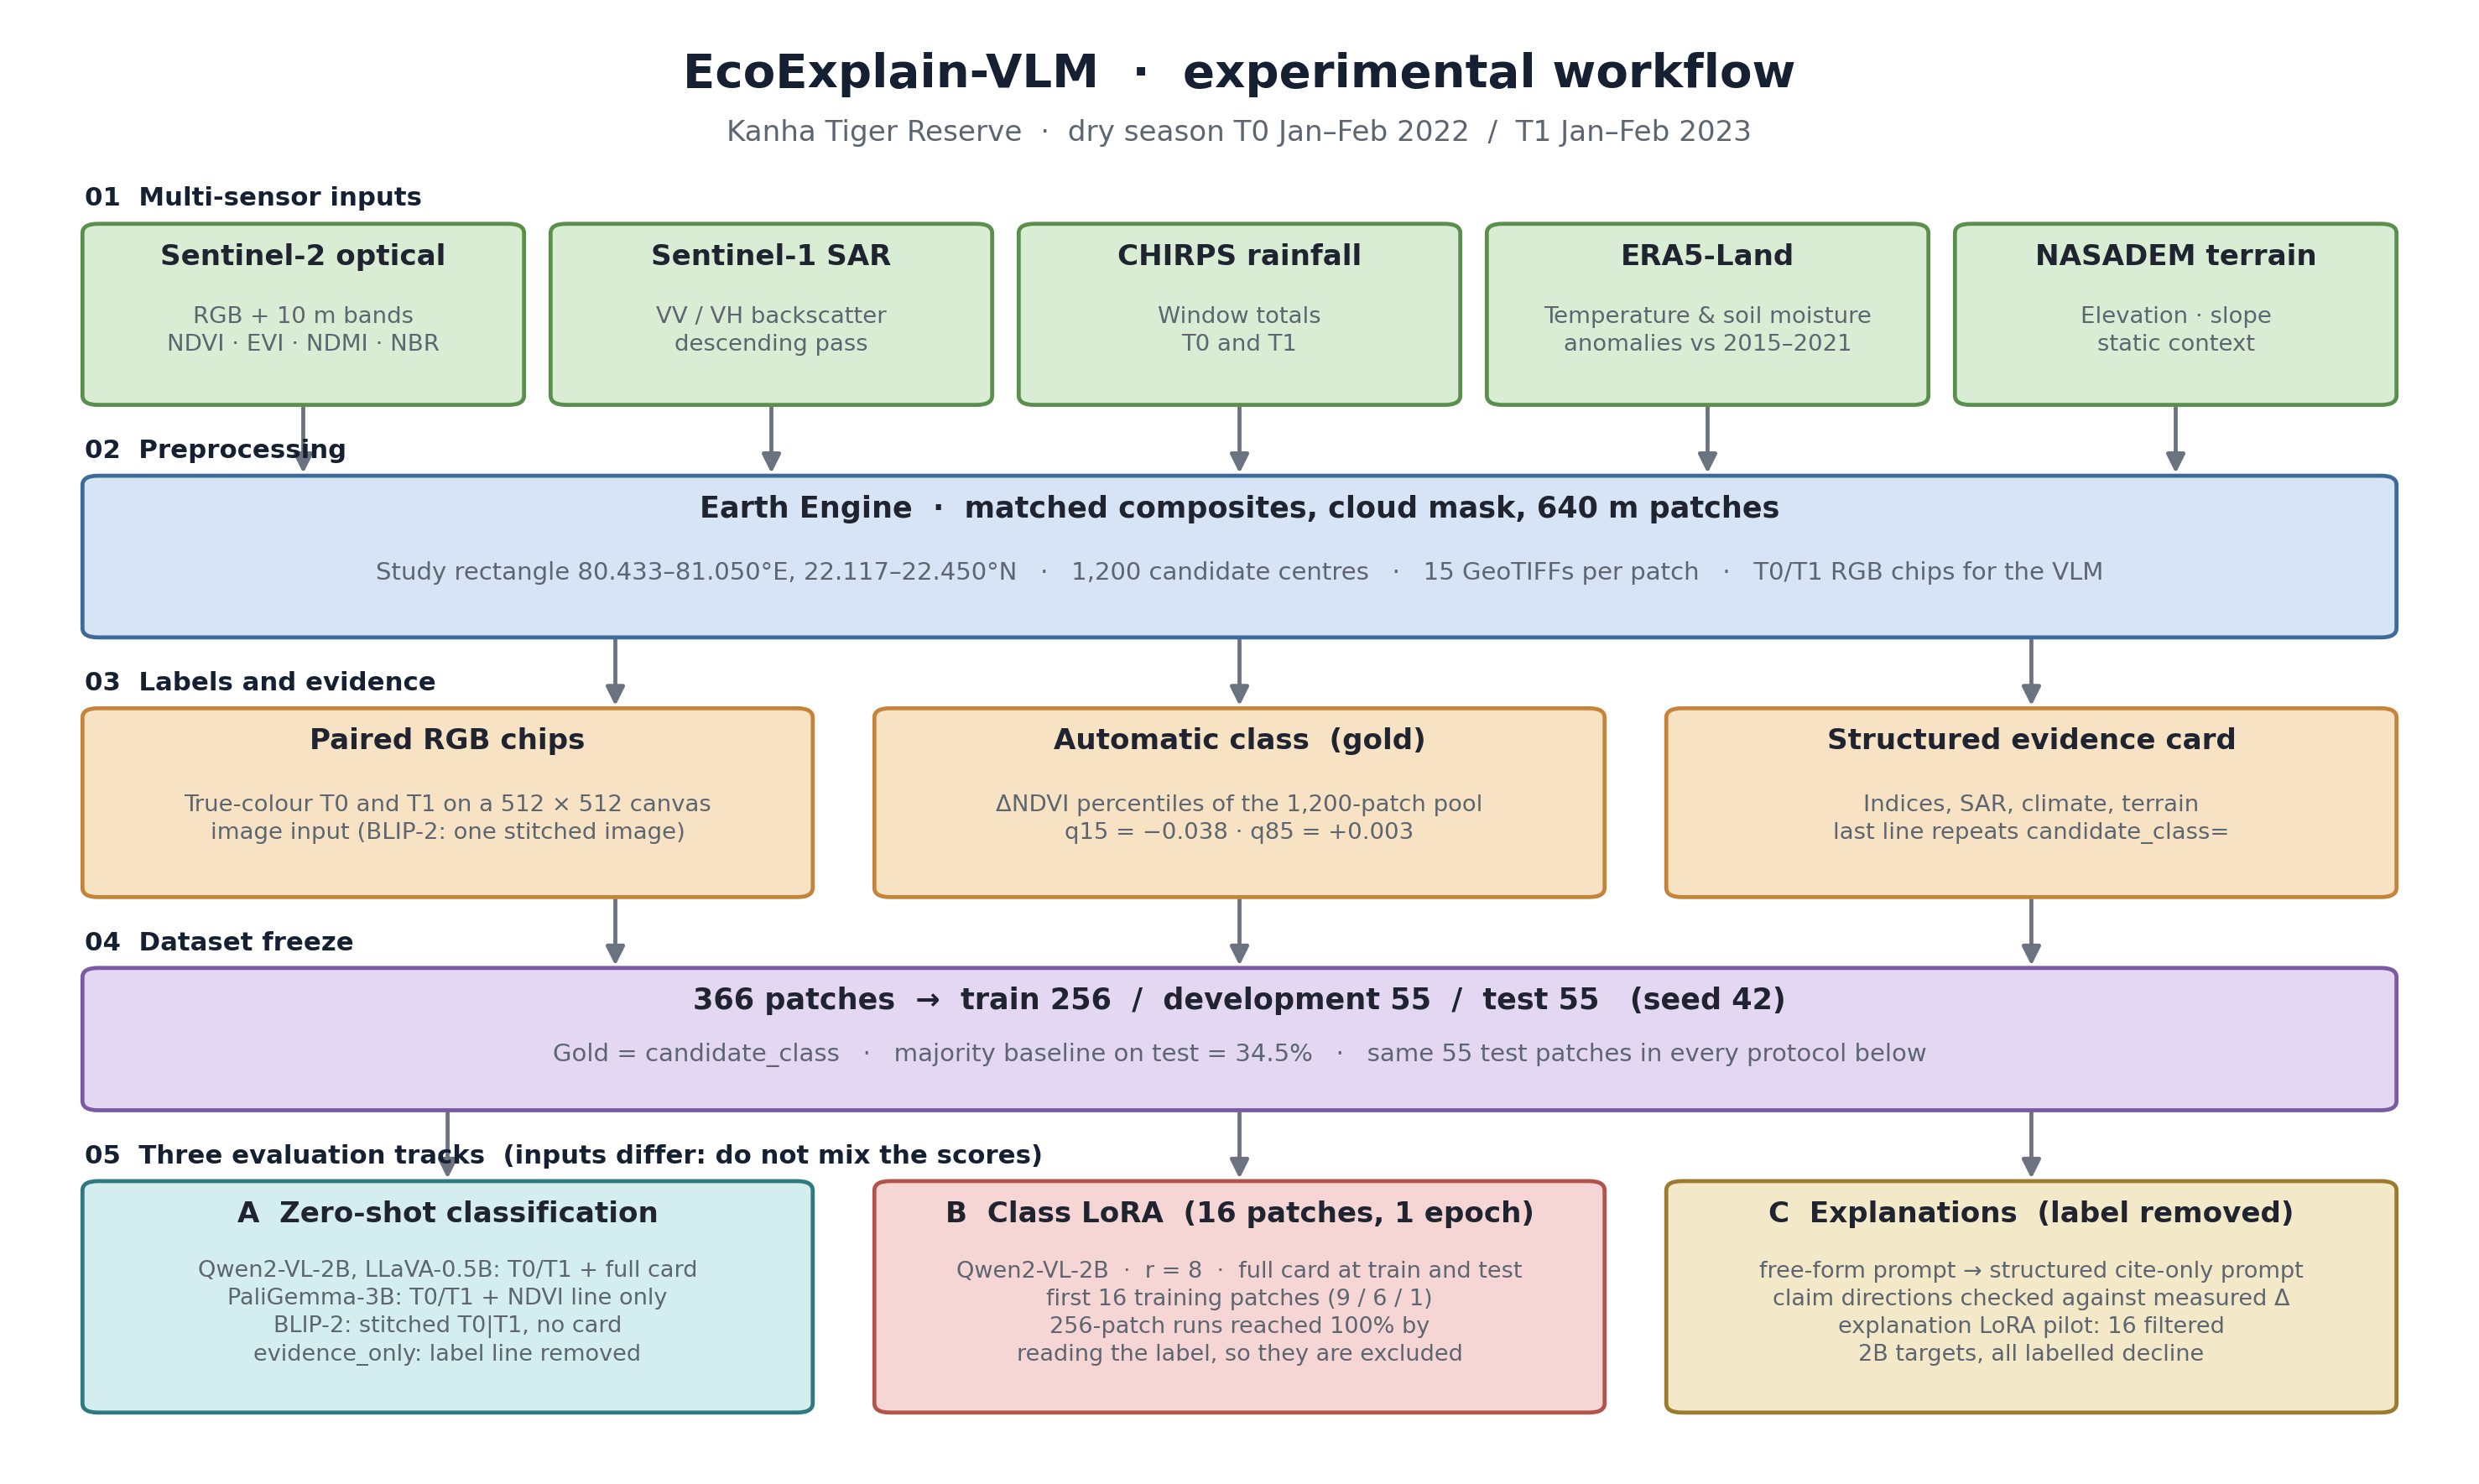
\includegraphics[width=\textwidth]{figures/fig_workflow_corrected.png}
\caption{The EcoExplain-VLM workflow. After the dataset is frozen, three
evaluation tracks run on the same 55 test patches and are scored
separately.}
\label{fig:workflow}
\end{figure*}

% ============================================================
% 3. RESULTS AND DISCUSSION
% ============================================================

\section{Results and Discussion}
\label{sec:results}

\subsection{Dataset Characteristics}

Table~\ref{tab:data} summarises the benchmark. The optical indices move
together: $\Delta$NDVI correlates with $\Delta$NBR, $\Delta$NDMI and
$\Delta$EVI at 0.80, 0.77 and 0.78. January-February 2023 was markedly
drier than 2022: mean window rainfall fell from 69.1 to 25.1\,mm, the
temperature anomaly rose from $-1.52$ to $+0.88$\,\textdegree C and the
soil-moisture anomaly fell from $+0.024$ to $-0.043$\,m$^3$/m$^3$; VV and
VH backscatter fell by 0.47 and 0.48\,dB. These climate and radar
signals are nearly identical across the three classes, so they describe
the year rather than individual patches, a useful property when judging
whether an explanation's causal claims are supported.
Figure~\ref{fig:ndvi} shows the label construction.

\begin{table}[t]
\centering
\small
\begin{tabular}{lr}
\toprule
Quantity & Value \\
\midrule
Candidate pool / final patches & 1,200 / 366 \\
Decline / stable / increase & 120 / 124 / 122 \\
Train / development / test & 256 / 55 / 55 \\
Test decline / stable / increase & 18 / 18 / 19 \\
Majority baseline (test) & 34.5\% \\
Spatial split train / dev / test & 266 / 46 / 54 \\
Mean $\Delta$NDVI (s.d.) & $-0.016$ (0.027) \\
Patches with $|\Delta\mathrm{NDVI}|\ge0.05$ & 34 \\
Human agreement & 8 / 19 (42\%) \\
\bottomrule
\end{tabular}
\caption{EcoExplain-VLM at a glance.}
\label{tab:data}
\end{table}

\begin{figure}[t]
\centering
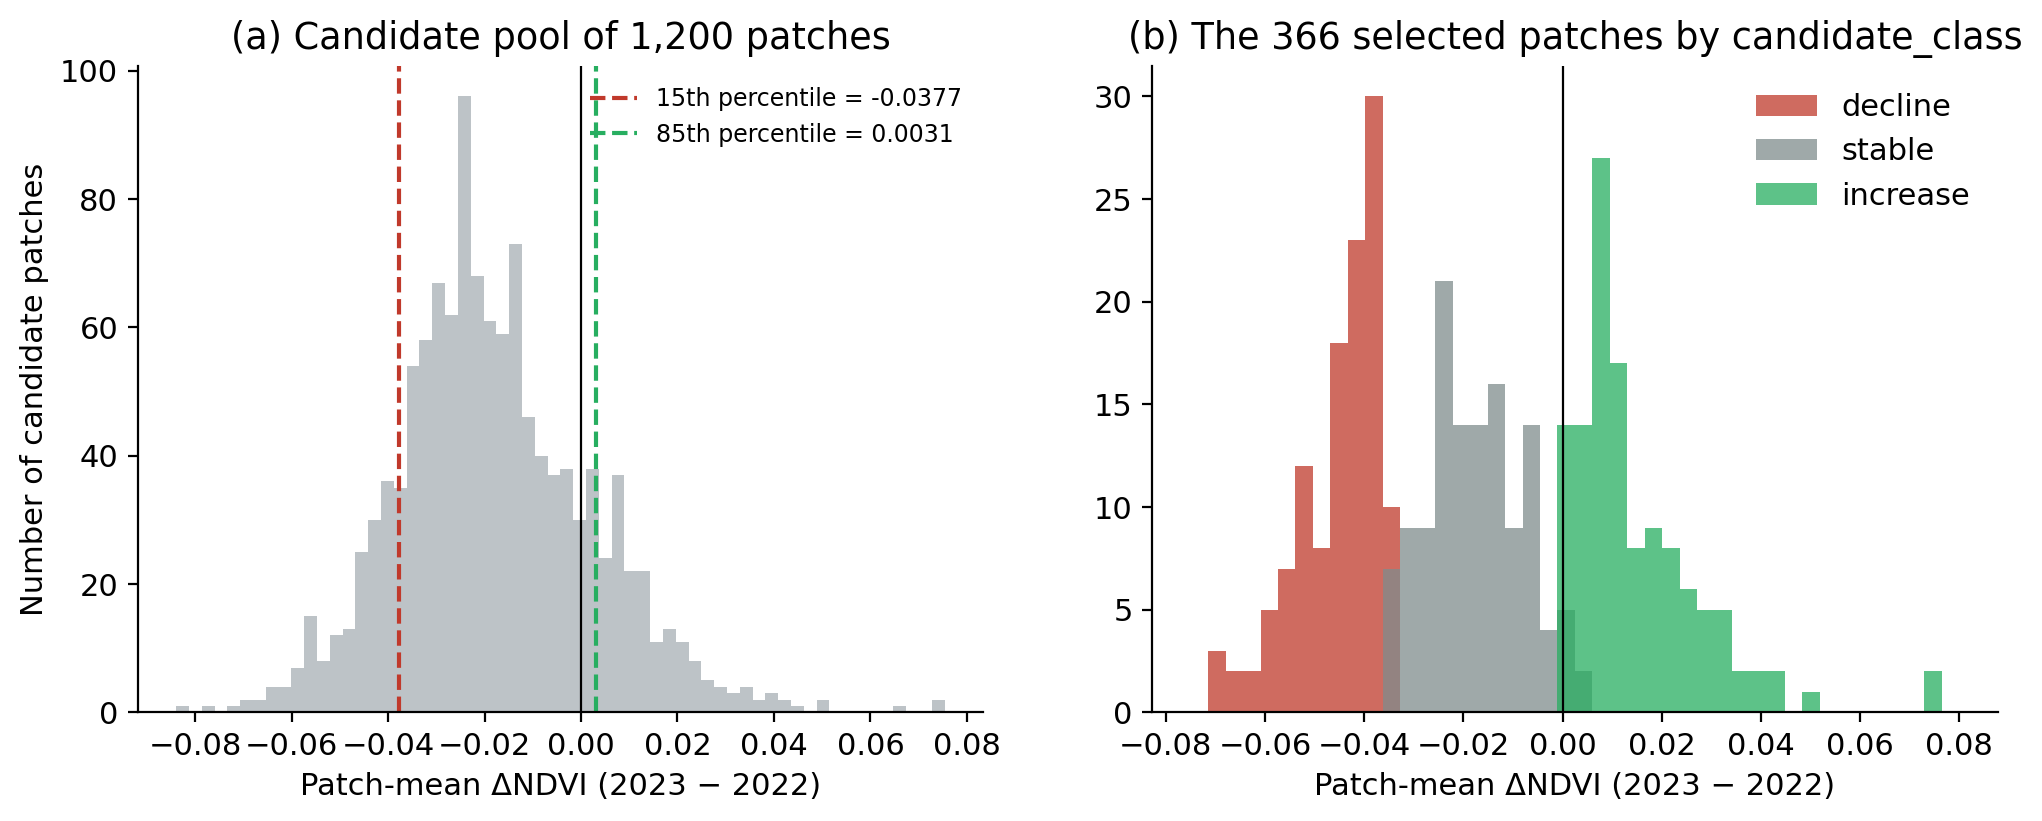
\includegraphics[width=\columnwidth]{figures/fig_ndvi_labels.png}
\caption{(a) Patch-mean $\Delta$NDVI over the 1,200-patch pool with the
15th and 85th percentiles. (b) $\Delta$NDVI of the 366 selected patches
by class.}
\label{fig:ndvi}
\end{figure}

\subsection{Zero-Shot Model Performance}

Table~\ref{tab:zeroshot} reports Track~A in two blocks. With the full
card, Qwen2-VL-2B reaches 56.4\% (95\% interval 43.3-68.6\%), the
highest zero-shot score, while the other models stay near the 34.5\%
majority baseline. The leak-free protocol explains this result. Removing
the summary line lowers Qwen2-VL-2B to 32.7\% under both the
evidence-only card and the compact table, where it answers ``stable''
for every patch (Figure~\ref{fig:leakfree}). On the patches where the
two Qwen runs disagree, the full card is right 18 times and the compact
table 5 times ($p=0.011$). The trend words that Qwen followed with the
full card appear only in the summary line, so its full-card score
reflects that line rather than the measurements.

\begin{table}[t]
\centering
\small
\begin{tabularx}{\columnwidth}{Xrr}
\toprule
Model (input) & Acc. & 95\% CI \\
\midrule
\multicolumn{3}{l}{\emph{Leak-free}} \\
Qwen2-VL-2B (evidence-only) & 32.7 & 21.8-45.9 \\
Qwen2-VL-2B (compact) & 32.7 & 21.8-45.9 \\
LLaVA-0.5B (compact) & \textbf{43.6} & 31.4-56.7 \\
PaliGemma-3B (compact) & \multicolumn{2}{r}{not available$^a$} \\
BLIP-2 (compact) & \multicolumn{2}{r}{no parsable answer} \\
\midrule
\multicolumn{3}{l}{\emph{Full card (includes summary line)}} \\
Qwen2-VL-2B & 56.4 & 43.3-68.6 \\
PaliGemma-3B (NDVI line only) & 36.4 & 24.9-49.6 \\
LLaVA-0.5B & 32.7 & 21.8-45.9 \\
BLIP-2 (images only) & 32.7$^b$ & 21.8-45.9 \\
\midrule
\multicolumn{3}{l}{\emph{Reference points}} \\
Majority class & 34.5 & 23.4-47.7 \\
$\Delta$NDVI rule, $\pm0.02$ & 63.6 & 50.4-75.1 \\
$\Delta$NDVI rule, fitted on train & 94.5 & 85.1-98.1 \\
\bottomrule
\end{tabularx}
\caption{Zero-shot accuracy (\%) on the 55 test patches. $^a$Gated model,
not loaded in the leak-free run. $^b$Produced by an echoed prompt under
the original parser.}
\label{tab:zeroshot}
\end{table}

\begin{figure*}[t]
\centering
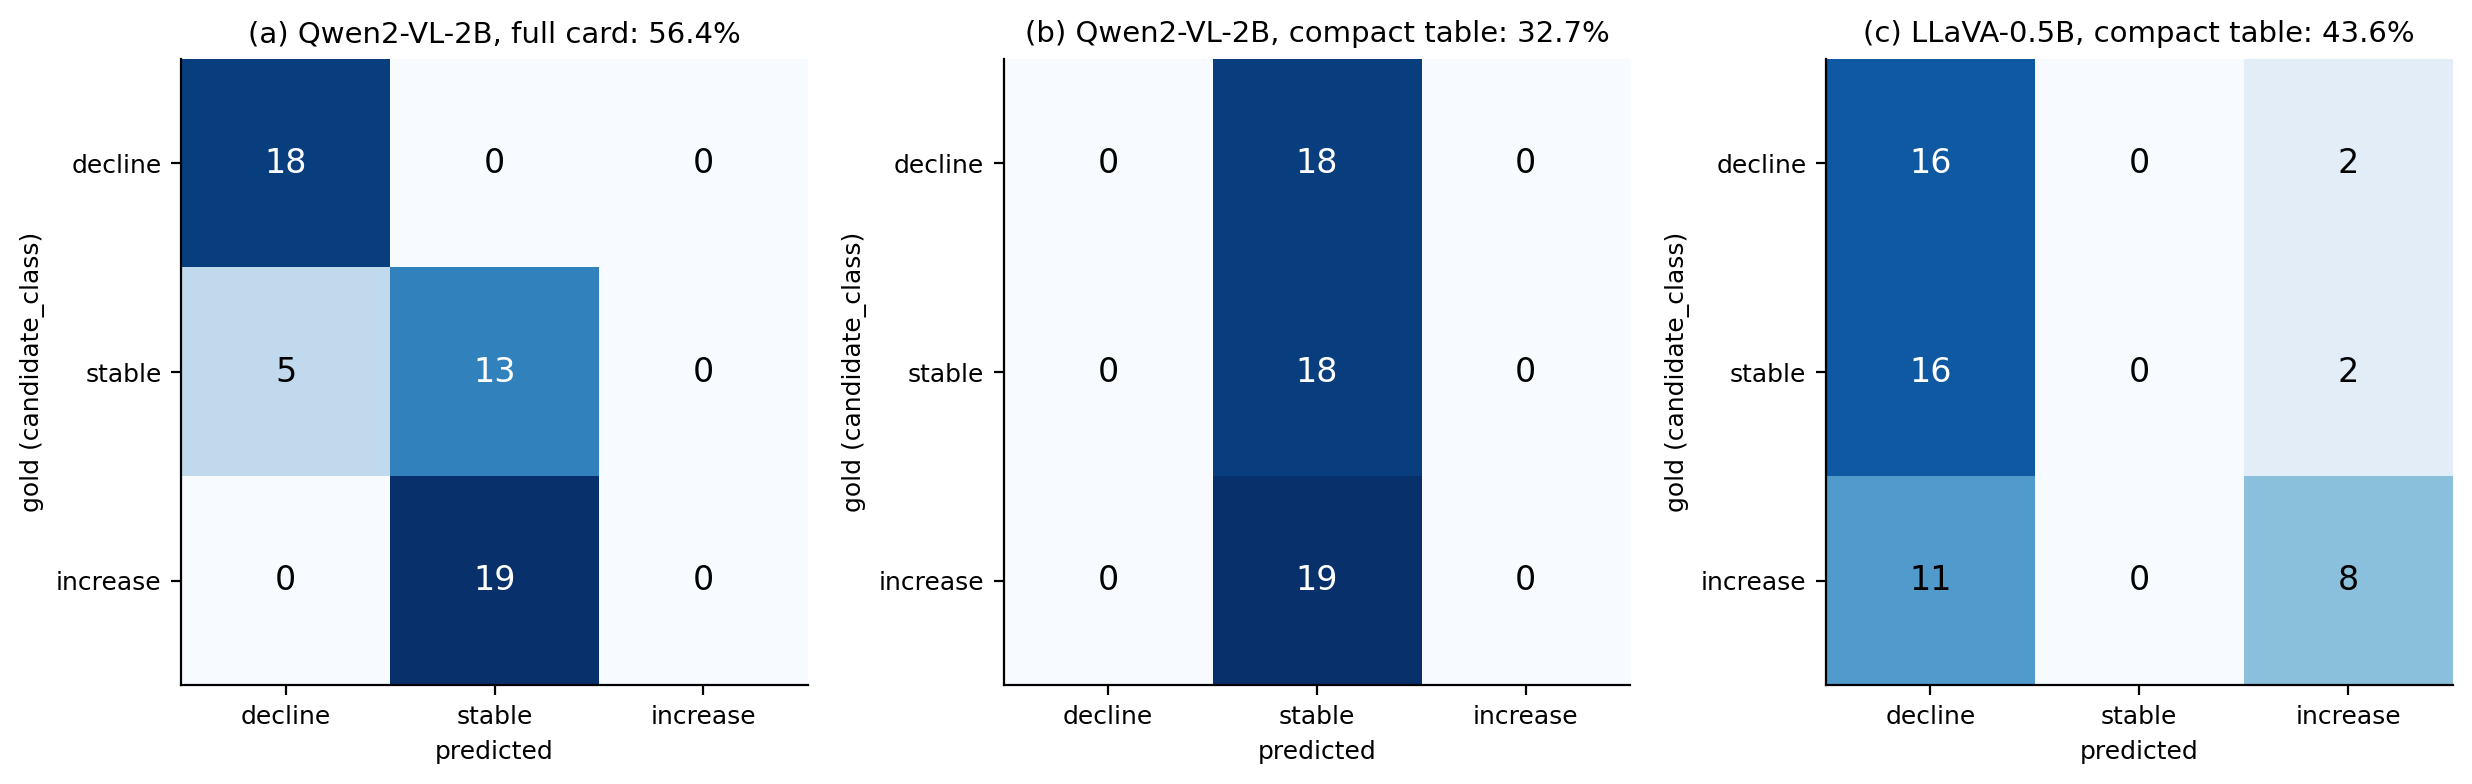
\includegraphics[width=0.85\textwidth]{figures/fig_leakfree_confusion.png}
\caption{Confusion matrices on the test set. (a) Qwen2-VL-2B with the
full card; (b) Qwen2-VL-2B with the label-free compact table; (c)
LLaVA-Interleave-0.5B with the compact table.}
\label{fig:leakfree}
\end{figure*}

The equal-input comparison is also informative. Given the same compact
table, LLaVA-Interleave-0.5B improves from 32.7\% to 43.6\%, recognising
16 of 18 decline and 8 of 19 increase patches. Its gain over the
baseline is not yet significant at $n=55$ ($p=0.44$), and it never
predicts ``stable'', but the change in behaviour shows that a cleaner,
numeric input helps the smaller model use the evidence.

The reference points place these results in context. A rule that reads
the single $\Delta$NDVI value on the card and applies two cut-offs fitted
on the training split classifies 94.5\% of the test patches correctly.
The information needed for the task is therefore present on every card;
what the small VLMs lack is the ability to extract and compare it. This
gap is a clear, measurable target for future models.

\subsection{Effect of Fine-Tuning}

The balanced, label-free class LoRA reaches 36.4\% (95\% interval
24.9-49.6\%; Figure~\ref{fig:lora}c). After one epoch on 16 examples
the adapter answers ``stable'' for 53 of 55 patches, which is close to
the zero-shot behaviour on label-free inputs ($p=0.50$) and to the
majority baseline ($p=1.0$). Earlier exploratory adapters trained with
the full card reached 67.3\% on 16 patches and 100\% on 256 patches, by
learning to read the label from the summary line
(Figure~\ref{fig:lora}b; Appendix~\ref{app:ft}); the leak-free protocol
correctly flags these as shortcut learning. The balanced run therefore
establishes a clean starting point: 16 examples are not enough to teach
the task, and the natural next step is a larger, balanced, label-free
fine-tune with early stopping.

\begin{figure*}[t]
\centering
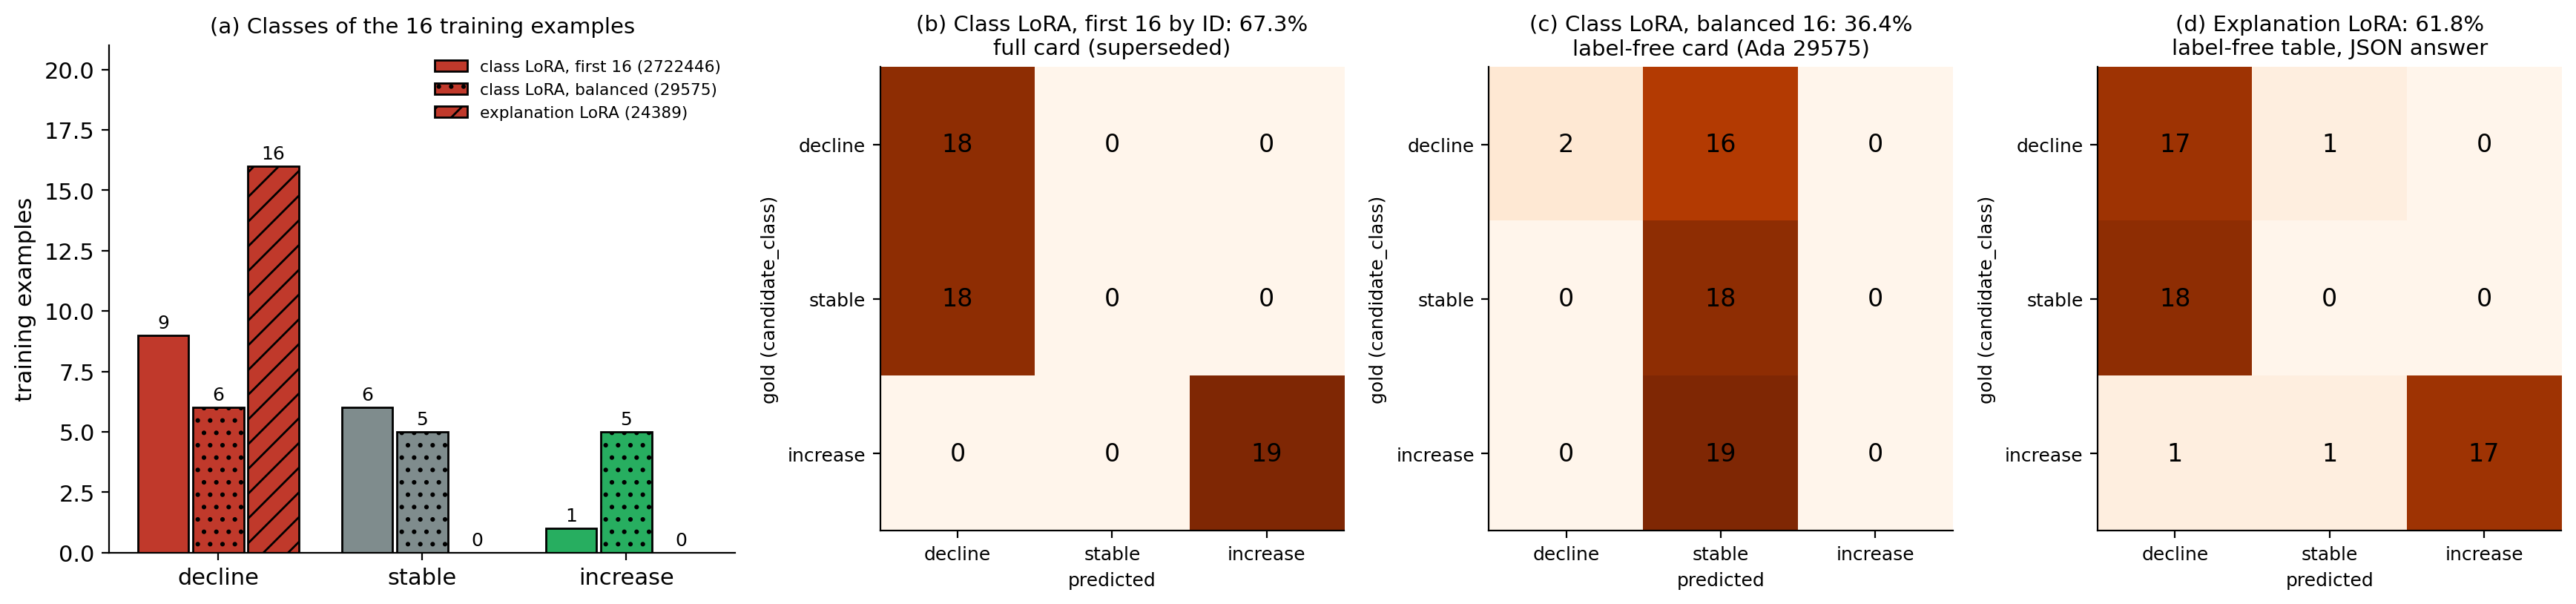
\includegraphics[width=\textwidth]{figures/fig_lora_v3.png}
\caption{Fine-tuning. (a) Class mix of the 16 training examples of each
adapter. (b) Exploratory class LoRA trained and tested with the full card.
(c) Balanced, label-free class LoRA. (d) Explanation LoRA, evaluated in
explanation mode.}
\label{fig:lora}
\end{figure*}

\subsection{Error Analysis}

Errors concentrate where the labels are weakest. Because the region
became slightly less green overall, many ``increase'' patches changed
NDVI by less than 0.011, and with the full card Qwen2-VL-2B labelled all
19 of them ``stable''. Each model also shows a characteristic default
answer in the leak-free setting (``stable'' for Qwen2-VL-2B and the
class LoRA; mostly ``decline'' for LLaVA). A
closed-set probe that scores each class word and corrects these
preferences with a development-set bias raises LLaVA to 60.0\%
(Appendix~\ref{app:results}), which points to calibration as a promising
remedy.

Part of the disagreement lies in the labels themselves. The card's own
trend words, computed with fixed thresholds, disagree with the
percentile label on 108 of 366 patches, and the human check confirmed
only 3 of 10 automatic ``increase'' labels. Some ``errors'' are thus
borderline cases rather than model failures, and the test labels were
not adjusted after seeing any model output.

\subsection{Explanation Quality}
\label{sec:expl}

Track~C asked the models to justify their answers using the label-free
compact table (Table~\ref{tab:explain}, Figure~\ref{fig:explain}). Under
a free-form prompt, PaliGemma and BLIP-2 gave no checkable reasons and
LLaVA's claims were correct 56.7\% of the time.

The structured cite-only prompt lists the facts the model may use,
states an NDVI decision rule, and asks for a one-sentence justification.
It raises claim correctness to 75.8\% for Qwen2-VL-2B and 71.1\% for
LLaVA, with self-consistency of 100\% and 90.7\%. Most claims still
flagged as incorrect (35 of 38 for Qwen, 35 of 37 for LLaVA) describe
true changes smaller than the scorer's dead-band rather than invented
facts. The justifications largely restate the supplied
facts and Qwen's class follows the stated rule on 53 of 55 patches, which
makes the explanations reliable but not yet interpretive.

\begin{table}[t]
\centering
\small
\begin{tabularx}{\columnwidth}{Xrrr}
\toprule
Setting & Class acc. & Correct claims & Self-cons. \\
\midrule
Free-form, LLaVA & 29.1 & 56.7 & 10.3 \\
Structured, Qwen2-VL & 63.6 & \textbf{75.8} & 100 \\
Structured, LLaVA & 45.1$^a$ & \textbf{71.1} & 90.7 \\
Explanation LoRA, Qwen2-VL & \textbf{61.8} & 50.5 & 96.4 \\
\bottomrule
\end{tabularx}
\caption{Explanation results (\%) on the test set with the label-free
table. $^a$Of 51 answered patches.}
\label{tab:explain}
\end{table}

\begin{figure*}[t]
\centering
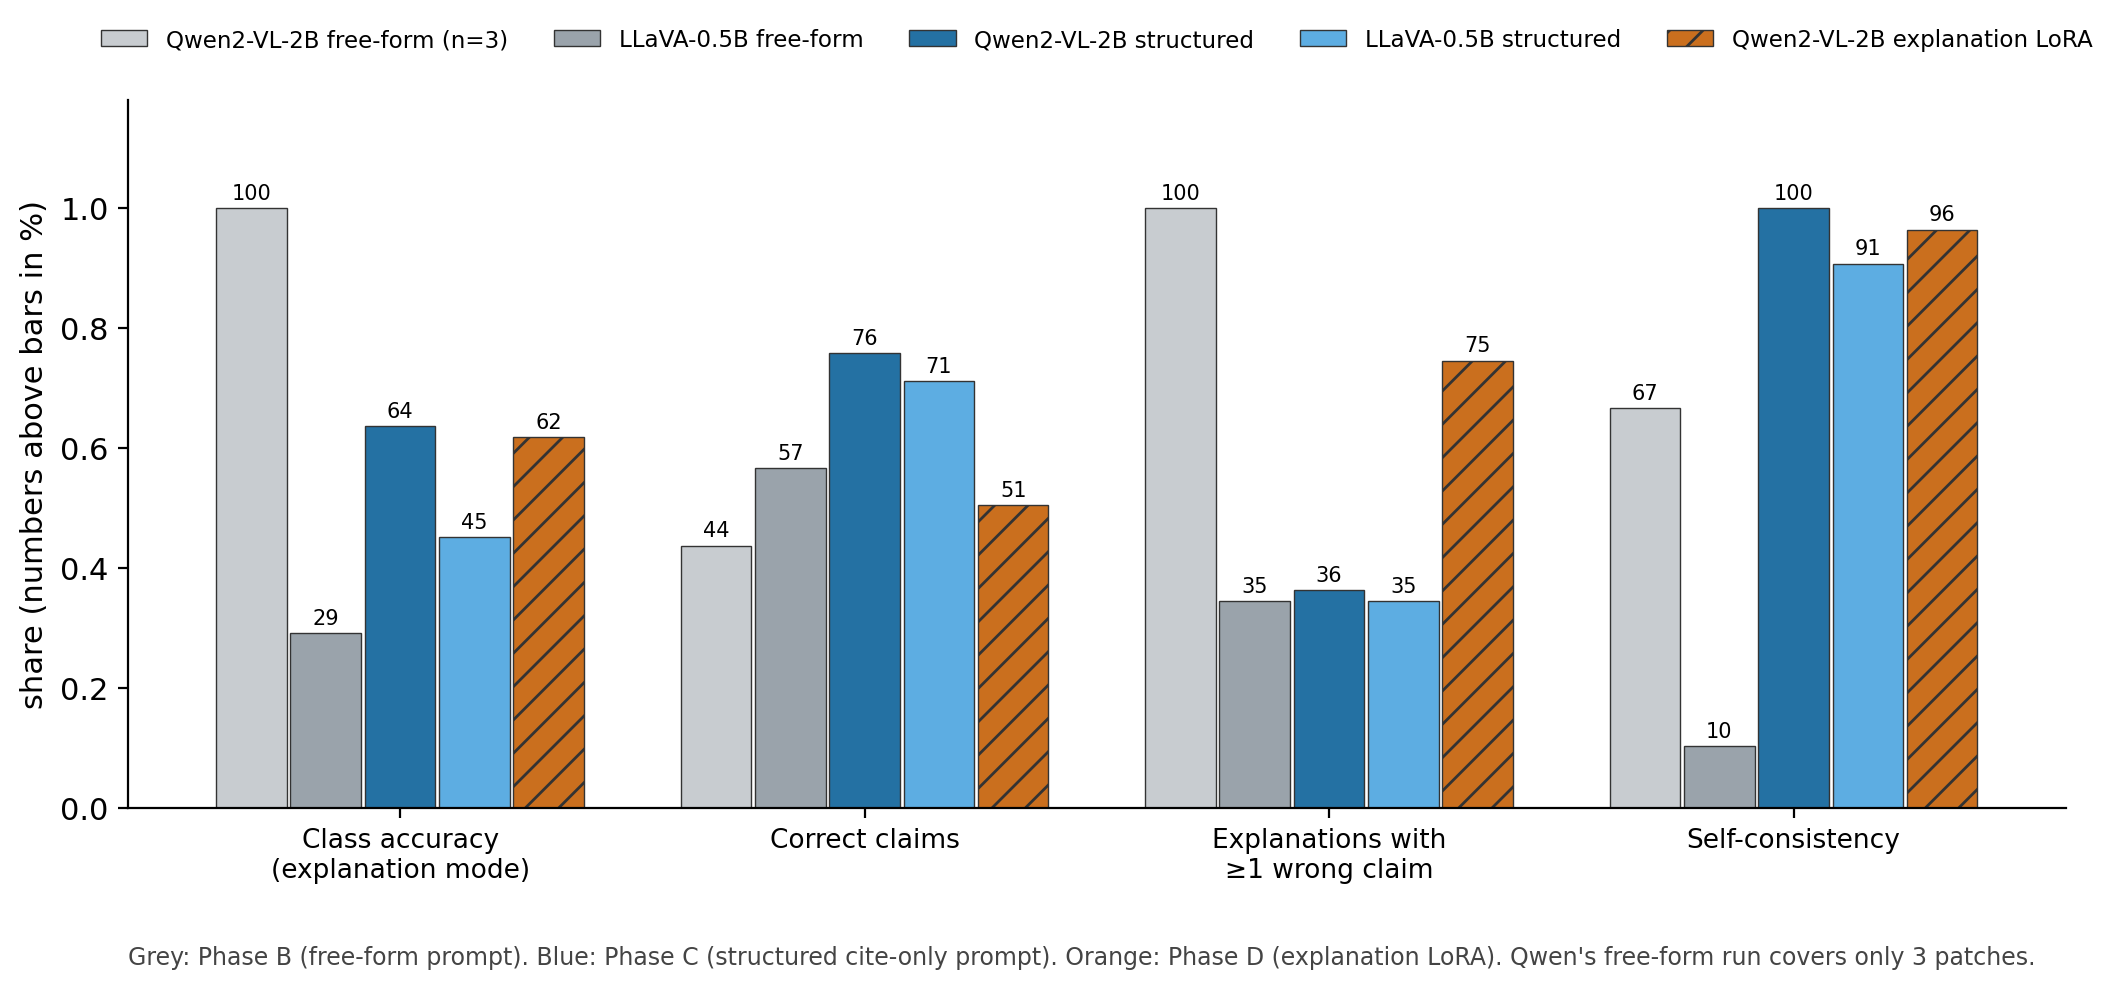
\includegraphics[width=0.9\textwidth]{figures/fig_explain_phases.png}
\caption{Explanation scores for the free-form prompt (grey), the
structured cite-only prompt (blue) and the explanation LoRA (orange).
The free-form Qwen2-VL-2B run covers three patches only.}
\label{fig:explain}
\end{figure*}

The explanation LoRA offers the most encouraging classification signal
in the study. Working from the label-free table without any stated rule,
it classifies 17 of 18 decline and 17 of 19 increase patches correctly
(61.8\%, interval 48.6-73.5\%), significantly above the majority
baseline (McNemar: 17 patches gained, 2 lost, $p<0.001$). It does not
yet recognise ``stable'' patches, and its claim correctness (50.5\%) is
below that of structured prompting, reflecting a small teacher set (16
examples, all labelled decline). Because the zero-shot counterpart of
this setting was run on only three patches, the relative contributions
of the prompt and of the fine-tuning remain to be separated; doing so is
a priority for follow-up work.

\subsection{Comparison with Existing Approaches}
 
Map-oriented change-detection methods provide excellent
wall-to-wall disturbance maps \citep{hansen2013}, and our threshold baseline confirms how
much information a single spectral index carries for this task.
Remote-sensing language datasets and
domain-adapted VLMs \citep{kuckreja2024} have shown that imagery and
language can be combined effectively. EcoExplain-VLM builds on these
advances by adding a new dimension: it tests whether a general VLM can
reason over the same multi-sensor evidence an analyst would use,
controls the input for label leakage, and verifies every directional
claim against measured values. CLIP-style encoders
offer efficient image-pair scoring, and EcoExplain-VLM complements them
by evaluating the written justification that makes a decision
transparent and checkable.


% ============================================================
% 4. CONCLUSIONS
% ============================================================

\section{Conclusions}
\label{sec:conclusions}

EcoExplain-VLM combines matched dry-season Sentinel-2 and Sentinel-1
data, climate and terrain context and a three-class vegetation-change
label into a reproducible benchmark for Kanha Tiger Reserve. Its
leakage-controlled protocol proved essential: the strongest zero-shot
result with the original card (Qwen2-VL-2B, 56.4\%) came from the card's
summary line, and with that line removed and inputs equalised, small open
VLMs remain near the majority baseline, with LLaVA-Interleave-0.5B best
at 43.6\%. A one-number rule reaching 94.5\% shows that the evidence is
sufficient, giving future models a clear target. For explanations, a
structured cite-only prompt makes more than 70\% of checkable claims
agree with the measured changes, and an explanation-tuned Qwen2-VL-2B
separates decline from increase without access to the label. Together,
the dataset, protocol and scoring tools give the community a practical
way to measure progress towards VLMs whose decisions about forest change
are both correct and verifiable.

% ============================================================
% LIMITATIONS (ACL: unnumbered, after the conclusions)
% ============================================================

\section*{Limitations}

\textbf{Image input.} The models only saw plain colour (RGB) images of
the forest, which look dark and almost the same in both years. They were
never shown the NDVI change maps or false-colour images, which show the
change much more clearly. Giving the models these more informative
images is a simple way they could perform better.

\textbf{Labels.} Our labels come from a simple rule on NDVI change
between two dry seasons, not from confirmed field data. Only one person
checked 19 patches by hand. Having several experts check more patches,
and measuring how often they agree (Cohen's $\kappa$), would make the labels more reliable.


\textbf{Fine-tuning.} Each fine-tuned model saw only 16 training
examples, once. Training on more examples with balanced classes, and
using a stronger model to write the training explanations, should give
a clearer picture of what fine-tuning can achieve.

\textbf{Evaluation tools.} Our explanation checker looks for key words
such as ``NDVI decreased''. It cannot understand negative sentences
such as ``NDVI did not decrease'', and it treats very small changes as
no change. Having people rate the explanations would add a useful
second check. The numbers on each evidence card are also slightly too
low (by about 8\%), because empty borders were included when averaging;
this is easy to fix.

% ============================================================
% REFERENCES
% ============================================================

% Bibliography in ACL format (acl_natbib), included here so no .bib file is needed.
\begin{thebibliography}{10}
\providecommand{\natexlab}[1]{#1}

\bibitem[{Drusch et~al.(2012)Drusch, Del~Bello, Carlier, Colin, Fernandez,
  Gascon, Hoersch, Isola, Laberinti, Martimort, Meygret, Spoto, Sy, Marchese,
  and Bargellini}]{drusch2012}
M.~Drusch, U.~Del~Bello, S.~Carlier, O.~Colin, V.~Fernandez, F.~Gascon,
  B.~Hoersch, C.~Isola, P.~Laberinti, P.~Martimort, A.~Meygret, F.~Spoto,
  O.~Sy, F.~Marchese, and P.~Bargellini. 2012.
\newblock Sentinel-2: {ESA}'s optical high-resolution mission for {GMES}
  operational services.
\newblock \emph{Remote Sensing of Environment}, 120:25-36.

\bibitem[{Gorelick et~al.(2017)Gorelick, Hancher, Dixon, Ilyushchenko, Thau,
  and Moore}]{gorelick2017}
Noel Gorelick, Matt Hancher, Mike Dixon, Simon Ilyushchenko, David Thau, and
  Rebecca Moore. 2017.
\newblock Google {Earth Engine}: Planetary-scale geospatial analysis for
  everyone.
\newblock \emph{Remote Sensing of Environment}, 202:18-27.

\bibitem[{Hansen et~al.(2013)Hansen, Potapov, Moore, Hancher, Turubanova,
  Tyukavina, Thau, Stehman, Goetz, Loveland et~al.}]{hansen2013}
M.~C. Hansen, P.~V. Potapov, R.~Moore, M.~Hancher, S.~A. Turubanova,
  A.~Tyukavina, D.~Thau, S.~V. Stehman, S.~J. Goetz, T.~R. Loveland, et~al.
  2013.
\newblock High-resolution global maps of 21st-century forest cover change.
\newblock \emph{Science}, 342(6160):850-853.

\bibitem[{Hu et~al.(2022)Hu, Shen, Wallis, Allen-Zhu, Li, Wang, Wang, and
  Chen}]{hu2022lora}
Edward~J. Hu, Yelong Shen, Phillip Wallis, Zeyuan Allen-Zhu, Yuanzhi Li, Shean
  Wang, Lu~Wang, and Weizhu Chen. 2022.
\newblock {LoRA}: Low-rank adaptation of large language models.
\newblock In \emph{International Conference on Learning Representations
  (ICLR)}.

\bibitem[{Jacovi and Goldberg(2020)}]{jacovi2020}
Alon Jacovi and Yoav Goldberg. 2020.
\newblock Towards faithfully interpretable {NLP} systems: How should we define
  and evaluate faithfulness?
\newblock In \emph{Proceedings of the 58th Annual Meeting of the Association
  for Computational Linguistics (ACL)}, pages 4198-4205.

\bibitem[{Kaufman et~al.(2012)Kaufman, Rosset, Perlich, and
  Stitelman}]{kaufman2012}
Shachar Kaufman, Saharon Rosset, Claudia Perlich, and Ori Stitelman. 2012.
\newblock Leakage in data mining: Formulation, detection, and avoidance.
\newblock \emph{ACM Transactions on Knowledge Discovery from Data},
  6(4):15:1-15:21.

\bibitem[{Kuckreja et~al.(2024)Kuckreja, Danish, Naseer, Das, Khan, and
  Khan}]{kuckreja2024}
Kartik Kuckreja, Muhammad~Sohail Danish, Muzammal Naseer, Abhijit Das, Salman
  Khan, and Fahad~Shahbaz Khan. 2024.
\newblock {GeoChat}: Grounded large vision-language model for remote sensing.
\newblock In \emph{Proceedings of the IEEE/CVF Conference on Computer Vision
  and Pattern Recognition (CVPR)}, pages 27831-27840.

\bibitem[{Li et~al.(2024)Li, Zhang, Zhang, Zhang, Li, Li, Ma, and
  Li}]{li2024interleave}
Feng Li, Renrui Zhang, Hao Zhang, Yuanhan Zhang, Bo~Li, Wei Li, Zejun Ma, and
  Chunyuan Li. 2024.
\newblock {LLaVA-NeXT-Interleave}: Tackling multi-image, video, and {3D} in
  large multimodal models.
\newblock arXiv:2407.07895.

\bibitem[{Tucker(1979)}]{tucker1979}
Compton~J. Tucker. 1979.
\newblock Red and photographic infrared linear combinations for monitoring
  vegetation.
\newblock \emph{Remote Sensing of Environment}, 8(2):127-150.

\bibitem[{Wang et~al.(2024)Wang, Bai, Tan, Wang, Fan, Bai, Chen, Liu, Wang, Ge
  et~al.}]{wang2024qwen2vl}
Peng Wang, Shuai Bai, Sinan Tan, Shijie Wang, Zhihao Fan, Jinze Bai, Keqin
  Chen, Xuejing Liu, Jialin Wang, Wenbin Ge, et~al. 2024.
\newblock {Qwen2-VL}: Enhancing vision-language model's perception of the world
  at any resolution.
\newblock arXiv:2409.12191.

\end{thebibliography}

% ============================================================
% APPENDIX
% ============================================================

\vfill\newpage % start the appendix at the top of the next column
\appendix
\section*{Appendix}

\section{Fine-Tuning Details}
\label{app:ft}

Table~\ref{tab:ftjobs} lists every class-LoRA run. The two full-card
runs on 256 patches reached 100\% with a training loss near zero,
consistent with reading the label from the summary line; the
16-patch full-card run used the first 16 training patches by
identifier (9 decline, 6 stable, 1 increase) and labelled every stable
patch ``decline''. These runs motivated the label-free, balanced
protocol used for the reported adapter.

\begin{table}[h]
\centering
\small
\begin{tabularx}{\columnwidth}{lrXr}
\toprule
Run & Train & Input (train / test) & Test \\
\midrule
Reported, balanced & 16 & label-free / label-free & 36.4 \\
Exploratory & 16 & full card / full card & 67.3 \\
Exploratory & 256 & full card / full card & 100 \\
Exploratory & 128 & full card / images only & 32.7 \\
\bottomrule
\end{tabularx}
\caption{Class-LoRA runs (accuracy in \%). All use $r=8$, $\alpha=16$,
one to three epochs, 4-bit Qwen2-VL-2B.}
\label{tab:ftjobs}
\end{table}

\section{Prompts and Output Parsing}
Qwen2-VL-2B and LLaVA received both images, protocol-specific card text, and a one-word classification instruction. 
PaliGemma used a text prompt identifying the T0 and T1 images, while BLIP-2 received side-by-side images and a short classification request. 
In the leak-free setting, BLIP-2 also received a compact evidence table. The explanation prompt specified permitted facts, the $\pm 0.02$ NDVI threshold, and a one-sentence justification. 
The parser extracted the first valid class label or synonym after removing echoed instructions.

\section{Additional Results}
\label{app:results}

A closed-set probe that scores each class word by its log-probability,
with a four-panel image, a stated NDVI rule and class biases fitted on
the development set, reached 60.0\% for LLaVA-Interleave-0.5B (it never
predicted ``stable''), against 32.7\% for PaliGemma and BLIP-2. In an
earlier label-free one-word run on 2 October, LLaVA scored 36.4\%. Under
the full card, a 128-patch adapter tested on images alone scored 32.7\%.
With $n=55$, all intervals are about $\pm13$ percentage points wide, so
per-class counts (about 18 patches per class) support only coarse error
analysis.

\end{document}
